\subsection{Эллипс}

{\bfseries \term{Эллипс}}~--- плоская замкнутая кривая, сумма расстояний от любой точки которой до двух фиксированных точек, называемых фокусами, постоянна.
\begin{equation}
	|F_1 M| + |F_2 M|=\const \label{eq:ell-def}
\end{equation}
\imp{Центром} эллипса называется середина отрезка, соединяющего его фокусы.

\imp{Большая ось} эллипса~--- прямая, проходящая через фокусы эллипса; \imp{малая ось}~--- прямая ей перпендикулярная и проходящая через центр эллипса.

\begin{wrapfigure}[10]{r}{0.5\tw}
	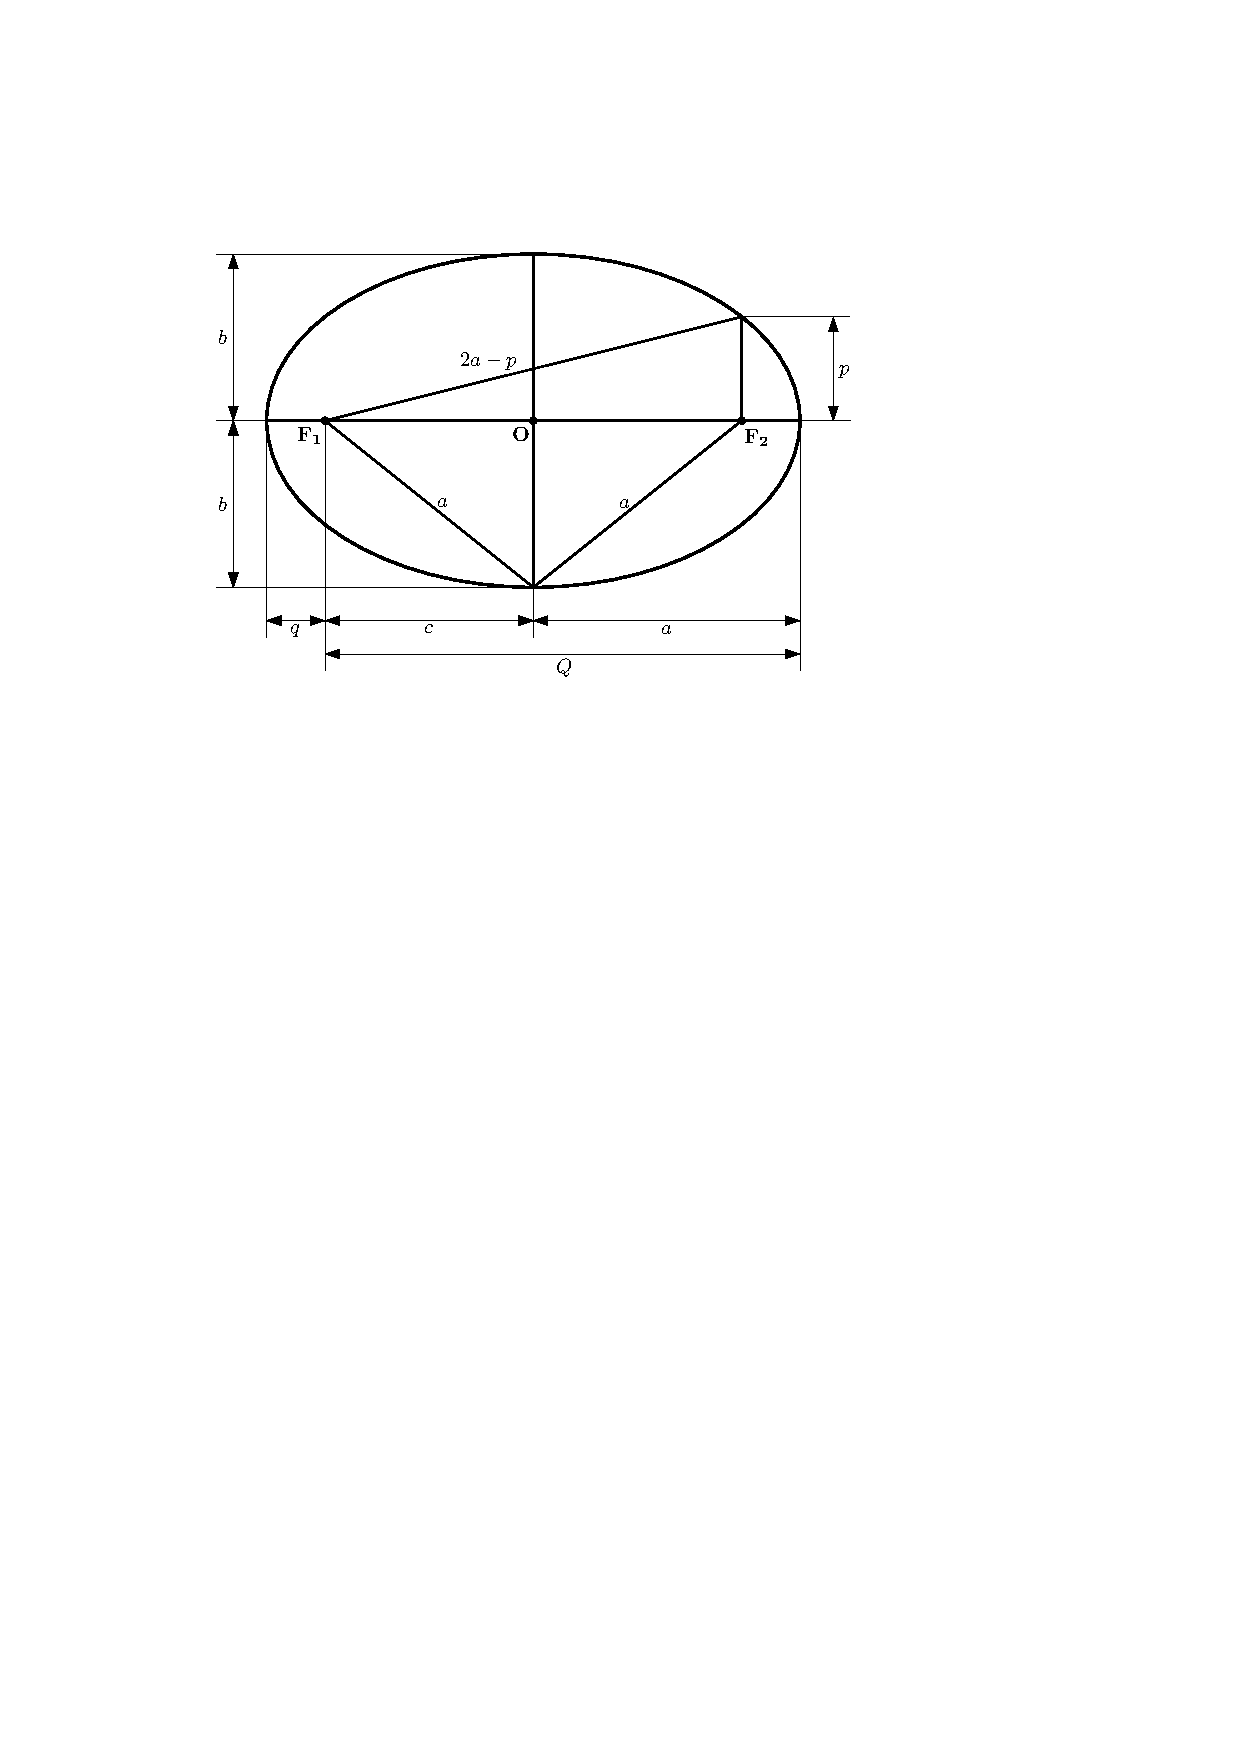
\includegraphics[width = .5\tw]{Ellips}
	\captionof{figure}{Эллипс}
	\label{pic:ellipse}
\end{wrapfigure}
Главные отрезки эллипса: \term{большая полуось} ($a$)~--- расстояние от центра эллипса до его пересечения с большой осью; \term{малая полуось} ($b$) определяется дословно также, заменив большую ось на малую; \term{фокальное расстояние} ($c$)~--- расстояние от центра эллипса до одного из фокусов, что тоже самое, половина расстояния между фокусами.

Рассмотрим крайнюю левую и крайнюю правую точки эллипса на Рис.~\ref{pic:ellipse}, назовем их $A$ и $B$ соответственно, тогда сумма расстояний $l$ от каждой из них до фокусов $F_1$ и $F_2$ равна:
\begin{equation*}
	AF_1 + AO + OF_2 = AF_1 + a + c = l = BF_2 + BO + OF_1 = BF_2 + a + c.
\end{equation*}
Откуда следует, что $A F_1 = B F_2$. Легко видеть, что $AB = 2a$, значит $l = AF_1 + AO + OF_2 = AO + OF_2 + F_2B = 2a$. Получается, сумма расстояний до фокусов от любой точки эллипса равна его удвоенной большой полуоси.

В силу равенства прямоугольных треугольников $\triangle F1 O C$ и $\triangle F_2 O C$ равны их гипотенузы $F_1C$ и $F_2C$, причем $F_1C= F_2C = l/2 = a$. Отсюда получается одно из основных соотношений в эллипсе:

\begin{equation}
	b^2 + c^2 = a^2.
\end{equation}
\term{Эксцентриситет} ($e$)~--- числовая
характеристика, показывающая степень отклонения конического сечения от окружности. Для эллипса $e$ лежит в интервале $(0, \, 1)$ и
определяется формулой
\begin{equation}
	e = \frac{c}{a}.
\end{equation}

\term{Апоцентр}~--- наиболее удаленная от заданного фокуса точка эллипса. Расстояние $Q$ до апоцентра от фокуса~--- сумма расстояний от фокуса, до центра эллипса и расстояния от центра до апоцентра, т.\,е.

\begin{equation}
	Q = c + a = a (1 + e).
\end{equation}

\term{Перицентр}~--- ближайшая точка эллипса к заданному фокусу. По аналогии с апоцентром, для расстояния $q$ от фокуса эллипса до перицентра справедливо следующее:
\begin{equation}
	q = a - c = a (1 - e).
\end{equation}

\term{Фокальный параметр}~($p$)~--- длина перпендикуляра, проведенного из фокуса до точки пересечения с эллипсом. Найдем $p$ из теоремы Пифагора для треугольника $\triangle F_1 F_2 P$:
\begin{gather}
	p^2 = (2a - p)^2 - (2c)^2, \notag\\
	p^2 =  4a^2 - 4ap + p^2 - 4a^2e^2,\notag\\
	0 = a ( 1 - e^2) - p,\notag\\
	p = a (1 - e^2) = \frac{b^2}{a} = b \sqrt{1 - e^2}.
\end{gather}

Получим теперь выражение для расстояния от произвольной точки эллипса с \term{истинной аномалией}~$\nu$~--- угол
{\slshape перицентр -- фокус -- заданная точка},
отсчитываемый в сторону движения по эллипсу. Для этого необходимо рассмотреть треугольник {\slshape перицентр -- фокус -- заданная точка} и записать для него теорему косинусов:
\begin{gather*}
	(2a - r)^2 = r^2 + (2c)^2 - 2 r \cdot 2c \cos (180^\circ - \nu),\\
	4a^2 - 4ar + r^2 = r^2 + 4 a^2 e^2 + 4 r a e \cos \nu,\\
	a - r = ae^2 + re\cos \nu,\\
	r = \frac{a(1 - e^2)}{1 + \cos \nu}.
\end{gather*}
Полученное выражение для длины радиус-вектора точки на эллипсе в зависимости от ее угла от перицентра называется \term{уравнением эллипса в полярных координатах}. Если же полюс системы координат расположить в другом фокусе, тогда полярный угол будет, очевидно, отсчитываться от точки апоцентра и в знаменателе уравнения будет знак <<$-$>>. Окончательно,
\begin{equation}
	r = \frac{a ( 1- e^2)}{1 \pm e \cos \nu}.
	\label{eq:ell-eq-pol}
\end{equation}

Перейдем теперь в декартовы координаты, в которых $r = \sqrt{x^2 + y^2}$, а $\cos \nu = x / r$, тогда:
\begin{gather*}
	\sqrt{x^2 + y^2} = \frac{a(1 - e^2)}{1 + e \cdot \dfrac{x}{\sqrt{x^2 + y^2}}} = \frac{a (1 - e^2) \sqrt{x^2 + y^2}}{\sqrt{x^2 + y^2} + e x},\\
	\sqrt{x^2 + y^2} = a(1 - e^2) - e x,\\
	x^2 + y^2 = a^2 (1 - e^2)^2 + e^2 x^2 - 2ae(1 - e^2) x,\\
	(1 - e^2) x^2 + y^2 = a^2 (1 - e^2)^2 - 2ae (1 - e^2) x,\\
	x^2 + \frac{y^2}{1 - e^2} = a^2 (1 - e^2) - 2aex.
\end{gather*}
Сдвинем систему отсчета влево так, чтобы центр эллипса оказался в начале координат, тогда новая координата по оси $x$ определяется, как $\xi = x + ae$, иначе $x = \xi - ae$. Подставим полученное выражение в преобразованное уравнение:
\begin{gather*}
	\xi^2 + a^2 e^2 - 2ae\xi + \frac{y^2}{1 - e^2} = a^2 (1 - e^2) - 2 ae\xi + 2 a^2 e^2,\\
	\xi^2 + a^2 e^2  + \frac{y^2}{1 - e^2} = a^2 - a^2 e^2 + 2 a^2 e^2,\\
	\frac{\xi^2}{a^2} + \frac{y^2}{a^2 (1 - e^2)} = 1,\\
	\frac{\xi^2}{a^2} + \frac{y^2}{b^2} = 1. \tag{\theequation} \label{eq:ell-eq-dec}
\end{gather*}
Данное уравнение называется \term{уравнением эллипса в декартовых координатах}.

Далее покажем, что любая точка плоскости, удовлетворяющая \eqref{eq:ell-eq-dec} принадлежит эллипсу с большой полуосью $a$ и малой~--- $b$, чтобы доказать равносильность предыдущих переходов. Для этого выберем произвольную точку $(x_0, y_0)$, для которой выполняется \label{eq:ell-eq-dec}, т.\,е.
\begin{equation}
	y_0 = \pm b \sqrt{1 - \frac{x_0^2}{a^2}} = \pm \sqrt{1 - e^2} \sqrt{a^2 - x_0^2}. \label{eq:ell-y0}
\end{equation}
Докажем, что множество точек $(x_0, y_0)$, для которых справедливо равенство \eqref{eq:ell-y0} являются эллипсом, а точки $(\pm a e, 0)$~--- его фокусами:
\begin{multline*}
	r_{1,2}
	= \big| (x_0, y_0) - (\pm ae, 0) \big|
	= \sqrt{(x_0 \mp ae)^2 + y_0^2} =\\
	= \sqrt{x_0^2 \mp 2 a e x_0 + a^2 e^2 + a^2(1 - e^2) - x_0^2(1 - e^2)} =\\
	= \sqrt{x_0^2 \mp 2 a e x_0 + a^2 e^2 + a^2 - a^2 e^2 - x_0^2 + e^2 x_0^2} = \\
	= \sqrt{e^2 x_0 \mp 2 a e x_0 + a^2 } = \sqrt{(e x_0 \mp a)^2} = |e x_0 \mp a| = a \mp ex_0.
\end{multline*}
Отсюда получается, что $r_1 + r_2 = 2a$, а значит рассмотренное множество точек, удовлетворяет определению эллипса. Это доказывает эквивалентность определений эллипса в виде \eqref{eq:ell-def}, \eqref{eq:ell-eq-pol} и \eqref{eq:ell-eq-dec}.

Теперь легко показать, что эллипс является образом афинного преобразования сжатия окружности с радиусом $a$. Для этого рассмотрим окружность, задаваемую уравнением $x^2 + y^2 = a^2$ и сжатие вдоль оси $y$ с коэффициентом $1/\sqrt{1 - e^2}$. Тогда $x' \hookrightarrow x$, а $y' \hookrightarrow y \sqrt{1-e^2}$. Следовательно для обратного преобразования $x \hookrightarrow x'$, а $y \hookrightarrow y'/\sqrt{1 - e^2}$. При этом прообраз сжатой окружность должен быть исходной окружность, а значит, удовлетворять исходному уравнения, то есть
\begin{gather*}
	x'^2 + \frac{y'^2}{1 - e^2} = a^2,\\
	\frac{x'^2}{a^2} + \frac{y'^2}{b^2} = 1.
\end{gather*}
Получаем, что образ окружности под действием афинного преобразования сжатия является эллипсом.

Данный факт помогает легко найти \term{площадь эллипса}~($S$)~--- площадь части
плоскости, ограниченной эллипсом. Так как под действием сжатия площади уменьшаются пропорционально коэффициенту преобразования, что есть
\begin{equation}
	S = S_\text{окр} \sqrt{1 - e^2} = \pi a^2 \sqrt{1 - e^2} = \pi a b.
\end{equation}

Также из свойств афинного преобразования и параметрического уравнения окружности следует \imp{параметрическое уравнение эллипса}, которое имеет такой вид:
\begin{equation}
	\left\{
	\begin{aligned}[lcl]
		&x=a\cos t,\\
		&y=b\sin t;\\
	\end{aligned}
	\right. \quad\quad t \in [0, \, 2\pi).
\end{equation}

Кроме этого, эллипс обладает важным \imp{оптическим свойством}, которое можно сформулировать так: свет от источника в одном из фокусов, отражается эллипсом так, что отражённые лучи пересекаются во втором фокусе или, что тоже самое, касательная к эллипсу в заданной точке образует с фокальными радиусами в данной точке равные острые углы. Для его доказательства необходимо показать равенство углов между касательной в точке к эллипсу и направлениями на фокусы. Для этого получим сначала уравнение касательной к эллипсу в произвольной точке $(x_0, y_0$, принадлежащей ему. Как было показано выше, эллипс можно представить объединением графиков двух функций \eqref{eq:ell-y0}. Найдем теперь производные от этих функций по $x_0$:
\begin{equation*}
	(y_0)'_{x_0} = \pm \sqrt{1 - e^2} \cdot \frac{-x_0}{\sqrt{a^2 - x_0^2}}.
\end{equation*}
Так как значение производной в точке равно тангенсу угла наклона касательной, то направляющий вектор касательной можно представить в виде $\vec{t} = \left(1,  (y_0)'_{x_0}\right)$, иначе:
\begin{equation*}
	\vec t =
	\begin{pmatrix}
		1\\
		\mp \sqrt{1 - e^2} \cdot \dfrac{\alpha}{\sqrt{1 - \alpha^2}}
	\end{pmatrix},~\text{где}~ \alpha \equiv \frac{x_0}{a},\quad -1 \leqslant \alpha \leqslant 1.
\end{equation*}
При этом модуль направляющего вектора $\vec t$ определяется, как
\begin{equation*}
	|\vec t| \equiv t = \sqrt{t_x^2 + t_y^2} = \sqrt{1 + (1 - e^2) \cdot \frac{\alpha^2}{1 - \alpha^2}} = \sqrt{\frac{1 - e^2 \alpha^2}{1 - \alpha^2}}.
\end{equation*}
Выпишем векторы $\vec r_1$ и $\vec r_2$, от точки $(x_0, y_0)$ до фокусов, имеющих координаты $(\pm ae, 0)$ соответственно:
\begin{equation*}
	\vec r_{1,2} =
	\begin{pmatrix}
		\pm ae - x_0\\
		-y_0
	\end{pmatrix}.
\end{equation*}
Покажем теперь, что $\cos \widehat{\vec r_1 \vec t} = - \cos \widehat{\vec r_2 \vec t}$ для верхнего полуэллипса, что завершит доказательство оптического свойства эллипса, так как для нижнего доказательство аналогично:
\begin{multline*}
	\cos \widehat{\vec r_{1, 2}  \vec t}
	= \frac{(r_{1, 2}, t)}{|\vec r_{1, 2}| | \vec t|} = \\
	= \frac{(\pm ae - x_0) \cdot 1 + \left[ -y_0 \cdot \left(- \sqrt{1 - e^2} \cdot \dfrac{\alpha}{\sqrt{1 - \alpha^2}} \right) \right]}{\sqrt{(\pm ae - x_0)^2 + y_0^2} \cdot \sqrt{\dfrac{1 - e^2 \alpha^2}{1 - \alpha^2}}} =\\
	= \frac{(\pm ae - x_0) \cdot \sqrt{1 - \alpha^2} + \alpha y_0\sqrt{1 - e^2}}{\sqrt{(\pm ae - x_0)^2 + y_0^2} \cdot \sqrt{1 - e^2 \alpha^2}}.
\end{multline*}
Из параметричекого уравнения эллипса можно получить, что $\sin t = x_0/a = \alpha$, тогда
\begin{equation*}
	y_0 = b \cos t = b \sqrt{1 - \sin^2 t} = b \sqrt{1 - \alpha^2} = a \sqrt{1 - e^2} \sqrt{1 - \alpha^2}.
\end{equation*}
Подставим данное выражение для $y_0$ в предыдущие выкладки:
\begin{multline*}
	\cos \widehat{\vec r_{1, 2}  \vec t}
	= \frac{a ( \pm e - \alpha) \sqrt{1 - \alpha^2} + \alpha a \sqrt{1 - e^2} \sqrt{1 - \alpha^2} \sqrt{1 - e^2}}{a \sqrt{(\pm e - \alpha)^2 + (1 - e^2)(1 - \alpha^2)} \cdot \sqrt{1 - e^2 \alpha^2}} = \\
	= \frac{ (\pm e - \alpha + \alpha - e^2 \alpha) \sqrt{1 - \alpha^2}}{\sqrt{e^2 \mp 2 e\alpha + \alpha^2 + 1 - \alpha^2 - e^2 + e^2 \alpha^2} \cdot \sqrt{1 - e^2 \alpha^2}} = \\
	= \frac{ (\pm e - e^2 \alpha) \sqrt{1 - \alpha^2}}{\sqrt{\mp 2 e\alpha + 1  + e^2 \alpha^2} \cdot \sqrt{1 - e^2 \alpha^2}} = \\
	= \frac{ e(\pm 1 - e \alpha) \sqrt{1 - \alpha^2}}{|1 \mp e\alpha| \sqrt{1 - e^2 \alpha^2}}
	= \frac{ e(\pm 1 - e \alpha) \sqrt{1 - \alpha^2}}{(1 \mp e\alpha) \sqrt{1 - e^2 \alpha^2}}
	= \pm \frac{e \sqrt{1 - \alpha^2}}{\sqrt{1 - e^2 \alpha^2}}.
\end{multline*}

